\documentclass[border=2mm]{standalone}

\usepackage{fontspec}
\usepackage{unicode-math}
\usepackage{amsmath}

\usepackage{pgfplots}
\pgfplotsset{compat=1.18}
\usetikzlibrary{arrows.meta, 
  calc, 
  positioning, 
  decorations.pathreplacing, 
  calligraphy}
\usetikzlibrary{patterns}

\usepackage{xcolor}
\definecolor{den-1}{HTML}{111111}   % Đen #111111
\definecolor{den-2}{HTML}{222222}   % Đen #222222
\definecolor{den-3}{HTML}{333333}   % Đen #333333
\definecolor{den-4}{HTML}{444444}   % Đen #444444
\definecolor{den-5}{HTML}{555555}   % Đen #555555
\definecolor{den-6}{HTML}{666666}   % Đen #666666


\begin{document}

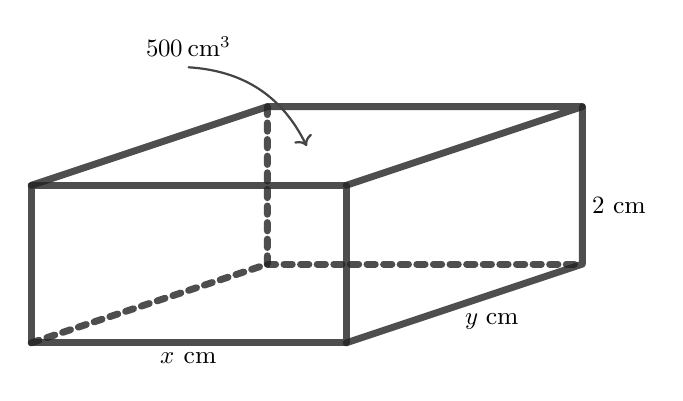
\begin{tikzpicture}[scale=1, line cap=round, line join=round]

  \draw [line width=2.5pt, color=den-2, opacity=.8] 
    (0,0) -- (4,0) -- (4,2) -- (0,2) -- cycle;
  
  \draw [line width=2.5pt, color=den-2, opacity=.8] 
    (0,2) -- (3,3) -- (7,3) -- (4,2);

  \draw [line width=2.5pt, color=den-2, opacity=.8] 
    (7,3) -- (7,1) -- (4,0);

  \draw [dashed, line width=2.5pt, color=den-2, opacity=.8] 
    (0,0) -- (3,1) -- (3,3);

  \draw [dashed, line width=2.5pt, color=den-2, opacity=.8] 
    (3,1) -- (7,1);

  % Nhãn
  \node at (2,0) [below] {\small $x$ cm};
  \node at (5.85,.5) [below] {\small $y$ cm};
  \node at (7,1.75) [right] {\small $2$ cm};

  % Mũi tên cong và ghi chú thể tích

  \draw [->, thick, color=den-4, rounded corners=10pt] 
    (2,3.5) to[bend left=30] (3.5,2.5);

  \node at (2,3.5) [above] {\small $500\,\text{cm}^3$};

\end{tikzpicture}


\end{document}
